\documentclass[a4paper, 11pt]{article}
\usepackage[T1]{fontenc}
\usepackage{lmodern}
\usepackage[utf8]{inputenc}
\usepackage{tikz}
\title{Implementing Bentley Ottmann}
\begin{document}
\maketitle
\section{Comparing paths}
\subsection{Segments}
\begin{figure}[htbp]
  \begin{center}
    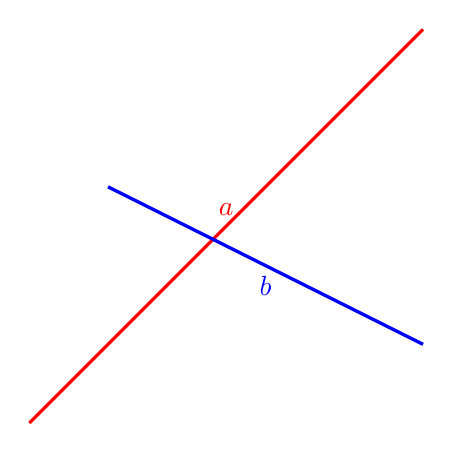
\begin{tikzpicture}
      \draw[very thick, draw=red] (0,0) edge node[above,text=red] {$a$} (5,5);
      \draw[very thick, draw=blue] (1,3) edge node[below,text=blue] {$b$} (5,1);
    \end{tikzpicture}
  \end{center}
  \caption{Is $a$ above $b$ ?}
  \label{fig:above}
\end{figure}

We maintain a set of alive paths during the whole algorithm.
This set requires to be sorted from topmost to bottom most.
An important question is therefore how to compare two different segments in order to
figure out which one is the topmost one.
We can see on Figure~\ref{fig:above} that most paths are not directly comparable.
Here we can see that on the left side $b$ is above $a$ while on the right side
$b$ is below $a$. Therefore which segment is the topmost one ?

The question as such is meaningless. In fact we need to add one more input and rephrase our
comparison question as : being given $a$, $b$ and a current position point $p$, which segment is
the topmost segment ?

\begin{figure}[htbp]
  \begin{center}
    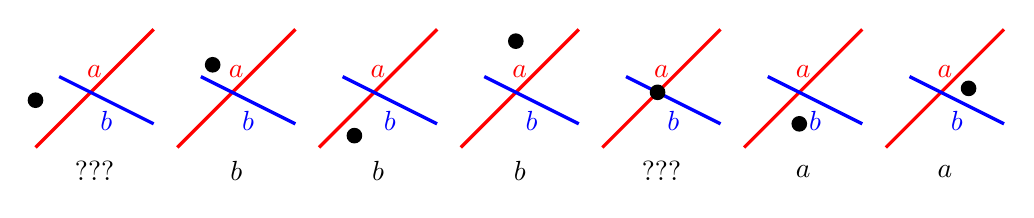
\begin{tikzpicture}[scale=0.3]
      \draw[very thick, draw=red] (0,0) edge node[above,text=red] {$a$} (5,5);
      \draw[very thick, draw=blue] (1,3) edge node[below,text=blue] {$b$} (5,1);
      \node[circle, fill=black, inner sep=2pt] at (0,2) {};
      \node at (2.5,-1) {???};
      \begin{scope}[xshift=6cm]
        \draw[very thick, draw=red] (0,0) edge node[above,text=red] {$a$} (5,5);
        \draw[very thick, draw=blue] (1,3) edge node[below,text=blue] {$b$} (5,1);
        \node[circle, fill=black, inner sep=2pt] at (1.5,3.5) {};
        \node at (2.5,-1) {$b$};
      \end{scope}
      \begin{scope}[xshift=12cm]
        \draw[very thick, draw=red] (0,0) edge node[above,text=red] {$a$} (5,5);
        \draw[very thick, draw=blue] (1,3) edge node[below,text=blue] {$b$} (5,1);
        \node[circle, fill=black, inner sep=2pt] at (1.5,0.5) {};
        \node at (2.5,-1) {$b$};
      \end{scope}
      \begin{scope}[xshift=18cm]
        \draw[very thick, draw=red] (0,0) edge node[above,text=red] {$a$} (5,5);
        \draw[very thick, draw=blue] (1,3) edge node[below,text=blue] {$b$} (5,1);
        \node[circle, fill=black, inner sep=2pt] at (2.333333,4.5) {};
        \node at (2.5,-1) {$b$};
      \end{scope}
      \begin{scope}[xshift=24cm]
        \draw[very thick, draw=red] (0,0) edge node[above,text=red] {$a$} (5,5);
        \draw[very thick, draw=blue] (1,3) edge node[below,text=blue] {$b$} (5,1);
        \node[circle, fill=black, inner sep=2pt] at (2.333333,2.333333) {};
        \node at (2.5,-1) {$???$};
      \end{scope}
      \begin{scope}[xshift=30cm]
        \draw[very thick, draw=red] (0,0) edge node[above,text=red] {$a$} (5,5);
        \draw[very thick, draw=blue] (1,3) edge node[below,text=blue] {$b$} (5,1);
        \node[circle, fill=black, inner sep=2pt] at (2.333333,1) {};
        \node at (2.5,-1) {$a$};
      \end{scope}
      \begin{scope}[xshift=36cm]
        \draw[very thick, draw=red] (0,0) edge node[above,text=red] {$a$} (5,5);
        \draw[very thick, draw=blue] (1,3) edge node[below,text=blue] {$b$} (5,1);
        \node[circle, fill=black, inner sep=2pt] at (3.5,2.5) {};
        \node at (2.5,-1) {$a$};
      \end{scope}
    \end{tikzpicture}
  \end{center}
  \caption{Which one is above ?}
  \label{fig:comparing}
\end{figure}

Fig.~\ref{fig:comparing} shows some expected answers for different positions.
Remark that it poses problem when the input position is exactly the intersection
of the two segments since the comparison becomes meaningless again.
To solve this problem we do the following~:
\begin{itemize}
  \item just before reaching the intersection, $b$ is above $a$ in our set.
  \item we the remove both segments.
  \item set the position to the intersection.
  \item re-inserts both segments with $a$ above $b$.
\end{itemize}

The meaning here is that being at the intersection is in fact being
right after meeting the intersection.

In order to ease the comparison process, we define a \emph{comparison\_key} function
taking a segment, a position and returning a key. Comparing two segments will then
only require comparing their corresponding keys.

We start by defining the segment angle as shown Figure~\ref{fig:angles}.
Consider a set of segments intersecting on a single point and position ourselves right
after the intersection. The topmost segment will have the smallest angle and the bottom-most
segment will have the largest angle.
Just before the intersection, the order is reversed.

\begin{figure}[htbp]
    \begin{center}
        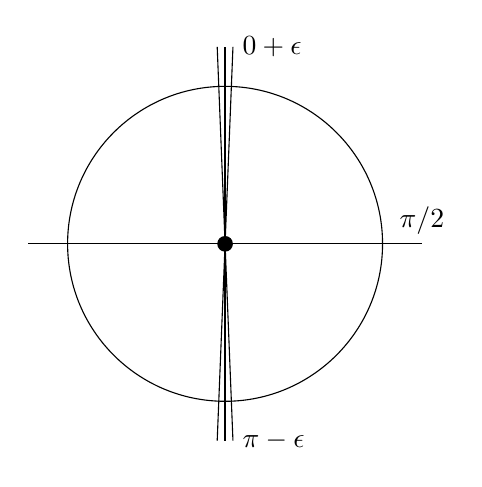
\begin{tikzpicture}[scale=0.5]
            \draw (0, 0) circle (4cm);
            \node[circle, fill=black, inner sep=2pt] at (0, 0) {};
            \draw[thick] (0, -5) to (0, 5);
            \draw (-0.2, -5) to (0.2, 5) node[right] {$0 + \epsilon$};
            \draw (-0.2, 5) -- (0.2, -5) node[right] {$\pi-\epsilon$};
            \draw (-5, 0) -- (5, 0) node[above] {$\pi/2$};
        \end{tikzpicture}
        \caption{segments angles}
        \label{fig:angles}
    \end{center}
\end{figure}


We therefore define the \emph{comparison\_key} function as follows:
\begin{itemize}
    \item it returns a tuple of two floating points values
    \item the first value is the $y$ coordinate of:
        \begin{itemize}
            \item if segment is not vertical then the intersection of cut line at current position and segment ;
            \item if segment is vertical then current position's $y$.
        \end{itemize}
    \item the second value is:
        \begin{itemize}
            \item if first value is less (or equal) than current position's $y$ then segment's angle
            \item else minus segment's angle
        \end{itemize}
\end{itemize}

We take a  small example to illustrate the behavior of the comparison key in a complex case.

Consider the three $a, b, c$ segments displayed on Figure~\ref{fig:keys}.

\begin{figure}[htbp]
    \begin{center}
        \begin{tikzpicture}
            \node (a1) at (0, 0) {$a_1$};
            \node (a2) at (3, 0) {$a_2$};
            \draw (a1) to (a2);
            \node (b1) at (1, 3) {$b_1$};
            \node (b2) at (1, -1) {$b_2$};
            \draw (b1) to (b2);
            \node (c1) at (0,2) {$c_1$};
            \node (c2) at (3, -1) {$c_2$};
            \draw (c1) to (c2);
        \end{tikzpicture}
    \end{center}
    \caption{Keys example}
    \label{fig:keys}
\end{figure}

We start initially at $a_1=(0,0)$. Only $a$ exists in the system, with a key of $(0, \pi/2)$.
We then continue with $c_1$ at position $(1, -3)$.
At this point, both $a$ and $b$ exist in the system.
Their keys are respectively of $(0, -\pi/2), (-3, \frac{3\pi}{4})$.
Next position is at $b_1=(1,-3)$. At this point the keys for $a, b, c$ are
$(0, -\pi/2), (-3, \pi), (-1, -\frac{3\pi}{4})$. Comparing the keys using lexicographical order
means $b$ is the topmost segment and $a$ the bottom-most.
We continue until arriving at the intersection of $b$ and $c$ at position $(1, -1)$.
At this point the keys become $(0, -\pi/2), (-1, \pi), (-1, \frac{3\pi}{4})$. $c$ is now above $b$.
Next stop is at the intersection of $a$ a and $b$ at $(1, 0)$.
Keys are now $(0, \pi/2), (0, \pi), (-1, \frac{3\pi}{4})$ and $a$ is now above $b$.
Next stop is $b_2$ where keys for $a$ and $c$ become $(0, \pi/2), (-1, \frac{3\pi}{4})$.
We reach the intersection of $a$ and $c$ at $(2, 0)$.
The key for $a$ is now $(0, \pi/2)$ and the key for $c$ is now $(0, \frac{3\pi}{4})$.
$a$ becomes top segment.

\end{document}
